\chapter[SCP-001 上帝的盲点]{
    SCP-001 God's Blind Spot\\
    SCP-001 上帝的盲点
}

\label{chap:SCP-001.gods.blind.spot}

\bb{项目编号:}SCP-001

\bb{项目等级:}Yesod

\bb{特殊收容措施:}T设施,基金会O5议会总部所在地及附属管理机构已围绕SCP-001所在地建立,包括SCP-001内的T-01号楼。T设施安保协议记录于文件T-001:01。

\begin{figure}[H]
    \centering
    \includegraphics[width=0.5\linewidth]{images/SCP-001-gods-blind-spot.jpg}
    \caption*{\bb{T设施}}
\end{figure}

\bb{描述:}SCP-001是一不规则形状空间,面积约65000平方米,包括地上和地下两部分,位于西奈山███████。除了其奇术性质(见下),SCP-001没有特殊之处,物质与能量可以自由出入其中。法国科学与艺术委员会在18世纪后期进行的考古研究表明此地有一石头建筑,可追溯到公元前2000年,类型符合住宿旅馆。由于T设施的建造,此原本建筑遗迹已无留存。

SCP-001的特殊之处,在于其为目前地球上已知唯一一处天然的Akiva辐射绝对零环境。实验已证实即便将Akiva辐射源引入SCP-001空间范围\footnote{参见研究报告SCP-001.08.P(佛陀齿遗物),1974。}的周围或内部此情况仍会维持,这表明并不仅是SCP-001的外边界严密阻隔了Akiva辐射穿过,SCP-001本身也在吸收和消灭发生于其内部的Akiva辐射。

作为SCP-001性质的结果,智人对象认知功能与器官功能的自然劣化、终结过程会在对象身处SCP-001边界内时中止。换句话说,在特定条件下,人类不会在SCP-001中死亡。参见下列测试记录:

\begin{longtable}{m{0.15\linewidth}m{0.6\linewidth}m{0.15\linewidth}}
\hline
\multicolumn{1}{c}{测试} & \multicolumn{1}{c}{参数} & \multicolumn{1}{c}{结果}\\
\hline
\endhead
\hline\multicolumn{3}{r}{\small{接下页}}
\endfoot
\hline
\endlastfoot
01.001 & 人员D-1082,健康人类男性,安置在SCP-001内部的标准收容间内,观察120天。 & 无变化。\\
01.003 & 人员D-2326,健康的人类女性,安置在SCP-001内部一气闭容器内。向容器内注入致命剂量氰化物气体,测试完成后将气体排出。 & D-2326未出现有害医疗问题。\\
01.006 & 参数同于测试01.003,但对象为30只健康的大白鼠(\ii{Rattus norvegicus})。 & 对象死于氰化物中毒。变体测试表明SCP-001的维生效应仅限于人类对象。\\
01.009 & 人员D-5337,患有4阶段癌症的人类女性(转移到大部分器官),预后其将立即死亡,将其安置在SCP-001内标准收容间中,观察786天。 & 无变化,身处SCP-001内期间对象的癌症症状无任何恶化。对象在测试结束离开SCP-001后的48小时内死亡。\\
01.010 & 人员D-5361,健康人类男性,将其安置在SCP-001内的焚化炉中然后启动。 & D-5361的身体如正常受控程序一样燃烧。其残骸没有特别之处。变体测试表明SCP-001的维生效应没有包括到全部类型的伤害。\\
01.338 & 人员D-8874,健康人类女性,安置在标准SCP-001内标准人形收容间中并被束缚。将对象的左腿在无麻醉下于大腿处截断,且不使用麻醉或止血带等束缚股动脉的措施。在截肢后,其断腿被移出SCP-001,对人员D-8874进行360天的观察。 & 对象暂时失去意识(可能是由于疼痛及突然失血)但恢复,流血在12小时内停止。截肢处快速愈合。移出SCP-001的断腿正常分解腐烂。\\
01.537 & 人员D-13926与D-13927,健康人类男性双胞胎,年龄24岁。D-13926安置于SCP-001内的标准长期人形收容间,D-13927安置在其他基金会设施的长期人形收容间。对象被观察26年零10月。 & 人员D-13927表现出正常的生理变化进程,而D-13926在测试期间没有出现明显衰老。测试结束后D-13926被送往其他基金会设施,这之后对象出现了加速发生的衰老变化。
\end{longtable}

已在T-01号楼内建造了居住设施,可供基金会O5议会全体成员和其他高级管理人员生活居住。当前,12名O5议会成员中有9人居于此宿舍内,此9人中的8人自T-01号楼建造完成起便再未离开。\footnote{第九位O5成员离开T-01号楼处理个人事务,在预定返回前遭气象事件杀死。}

因SCP-001的性质,其也被用作基金会奇术研究计划的控制站点,包括\hyperref[chap:SCP-2336]{SCP-2336-A个体}的应用开发。

\bb{归档文件06-S7INF-23-A(摘录)}

\begin{figure}[H]
    \centering
    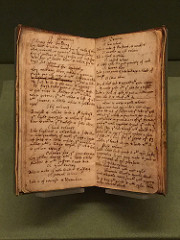
\includegraphics[width=0.5\linewidth]{images/SCP-001-gods-blind-spot-2.jpg}
    \caption*{\bb{手稿“对上帝实质的观察”(艾萨克·牛顿爵士)基金会收藏品。}}
\end{figure}

\begin{scpbox}

…在自然哲学和对全能上帝本质的问题上,我们必须凭着感官的证据开展探究,包括神圣经文的证词。虽然无人曾见得上帝,然而对上帝之感知可来自观察他的创造,及至对神圣经文的细致研究。

思考出埃及记第四章,以希伯来文写是:

\usefreeserif{ויהי בדרך במלון ויפגשהו יהוה ויבקש המיתו׃}

\usefreeserif{ותקח צפרה צר ותכרת את־ערלת בנה ותגע לרגליו ותאמר כי חתן־דמים אתה לי׃}

这,将其翻译,是说:

\ii{摩西在路上住宿的地方,耶和华遇见他,想要杀他。西坡拉就拿一块火石,割下他儿子的阳皮,丢在摩西脚前,说:“你真是我的血郎了。”}\footnote{出埃及记4:24–26}

思考这些诗篇的教导。许多饱学学者将关注点投于诗篇第二段,这里西坡拉,摩西之妻,施行割礼,且,以此做法,解救她的丈夫免于全能上帝的怒火。在此,学者们说,是一种道德教诲,告诉说没有人,即便是上帝的先知,得以豁免于他的约法。

但思考诗篇第一段,对此了解甚少。全能上帝,已经产生意图杀死摩西,试图如此却失败。这一段是理解上帝本质的关键。我们必须明白若经文是绝对可靠的,且经文在告诉我们全能上帝试图杀死摩西而未成,那么绝对可靠的经文就是在说上帝不是全能的,或至少说上帝的权柄延伸不到这片特定区域。

\bb{艾萨克·牛顿爵士,《对上帝实质的观察》(1734年)}

\end{scpbox}

\hr

\begin{figure}[H]
    \centering
    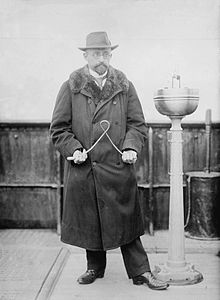
\includegraphics[width=0.5\linewidth]{images/SCP-001-gods-blind-spot-3.jpg}
    \caption*{\bb{便携式奇术仪器实验}}
\end{figure}

\begin{scpbox}

“…新近发明的奇术设备让我们的教团得以验证长期以来的怀疑,也即神恩-或者以我们某些兄弟更常用的称谓-奇术力–是一种真实的、可度量的实质现象。我的一位同事提出以“akiva”作为此现象的度量单位,来自某些死去很久的希伯来殉道者。这种哲学与技术突破激起了许多计划的启动,包括对全球akiva状况及变化的测绘。这可不是测绘尼罗河源、或是给无聊海岩命名那样的简单事-这份奇术地图将成为价值无量的工具,让我们的教团能利用神恩之力。

“于是,我们组织了制图队,每人配备一台奇术设备,来完成测绘计划,对值得特别关注的地区尤为注意。

“在圣地的某一角,拿破仑·波拿巴为我们指路了。如你们所知,拿破仑1798年在埃及的战役中有法国科学与艺术委员会参与,它们完成了对此国家的全面测量。\footnote{\ii{Description de l'Égypte, ou Recueil des observations et des recherches qui ont été faites en Égypte pendant l'expédition de l'armée française}}报告的第11卷中测绘了历史地点的地理方位,包括圣经中的何烈山。由此,在这份情报的鼓动下,一队共济会及我们秘教团成员,由我带领,动身去往西奈山,重走摩西从何烈山回到法老宫廷的征途。

今夜,我很高兴地报告教团的努力有了成果。我们找到了‘路上住宿的地方’。”

\bb{布拉姆·史托克}\footnote{译注:爱尔兰作家,著名作品是吸血鬼小说《德古拉》;对超自然颇有兴趣,和黄金黎明相关人士有密切交往,但没有他本人明确入会的记载。}\bb{,抄录自黄金黎明秘教团会议备忘录(1874)}

\end{scpbox}

\hr

\begin{figure}[H]
    \centering
    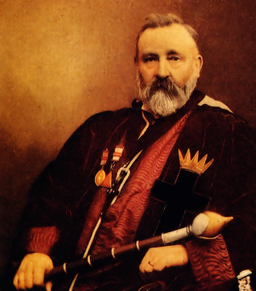
\includegraphics[width=0.5\linewidth]{images/SCP-001-gods-blind-spot-4.png}
    \caption*{\bb{威廉·永利·韦斯科特(基金会档案照片)}}
\end{figure}

\begin{scpbox}

\bb{站点主管威廉·永利·韦斯科特}\footnote{韦斯科特合作创立了基金会的前身组织之一。}\footnote{译注:威廉·永利·韦斯科特,共济会成员,黄金黎明会社的创始人之一}\bb{至Samuel Liddell Mathers的备忘录摘录,1916年10月16日}

…在住宿地研究、测试其性质后,结论只有一个。上帝也有盲点,我们找到了它。

不仅是躲避死亡天使,住宿地的性质能为多种奇术工程带来机遇。我们现在知道Akiva背景辐射等级在住宿地内无论如何都是零。这就意味着,既然这是上帝的盲点,任何在其范围内做出的举动都不会有神学上的后果。我非物理学家,但我们的同事尼古拉已经把它描述成了罪恶的法拉第笼。将此地用作中心决策的总部的适宜性-成为我们新教团的主体,显然是再明显不过的了。

\end{scpbox}

(备注:自建立起,基金会伦理委员会便一直设置于T-01号楼。)

\hr

\begin{scpbox}

\bb{马尔文·斯克兰顿博士的笔记,1924年7月31日(摘录)}

…作为我们对SCP-001性质的研究结果,我们现已准备在Site-36这里开展第一次人造Akiva真空屏障实验,我们称之为反胞体。基本上我们要创造的就是另一个SCP-001。今日的测试将是二十余年奇术工程及应用神学的巅峰。Bertrand,我的助理,说的更为直率:我们要造个盒子,然后把上帝从里面扔出去…

…

结果是自然厌恶真空,也厌恶内禀。我们的仪器读数表明当反胞体启动,测试胶囊内的可测量Akiva倒是降到了零,休谟等级却飙升了。我们觉得有其他东西-我们现在还没法观察测量-进来了。我们不知道那是什么或者要去何方…

\end{scpbox}

\hr

\begin{scpbox}

\bb{O5政策备忘K-308(1924年8月2日)(摘录)}

先生们:

自7月31日Site-36的事故以来,异常事件的频率与烈度开始猛烈增高;\footnote{虽然其与反胞体测试的因果关系尚无可信验证,其时间值得注意。}如我们所讨论的,这种情形使基金会必须重修和扩张使命宪章。目前我们已经是一个研究组织。但紧急时刻需要紧急措施,已经有必要让我们的团体不至于收容研究生物了。我们必须迈出步伐,控制尚未被基金会取得的异常,即是为了保证异常不被更多研究,也是为了保护全人类。

基金会在此批准成立活动外勤行动部门,立即生效。现存的研究活动就此改组为包含独立的不同研究部门。在此授权这一新机构部门立即组建、投资、招募、装备、训练与部署一或多支机动特遣队。外勤行动部门的临时领导及预算列于附录展示…

\end{scpbox}

(备注:备忘K-308是基金会不再止步于研究、而是积极收集与收容异常项目、实体与现象的正式开端。)

\hr

\begin{scpbox}

\bb{备忘}

\bb{至:管理员;O5议会}\\
\bb{副本抄送:Muhammad al-Taqi主管(战略神学办公室)}\\
\bb{自:Sheldon Katz先生}\\
\bb{日期:19██年8月3日}

Re: 谈判状况(乌列尔计划)

我相信我们已经与对方达成了理解。本备忘的目的是记录理解之要目。如我们所讨论的,正式合约会以协约的形式呈现。\footnote{预期为石板,但我已要求提供PDF文件。}

\uu{背景}

基金会在T设施的行动已多次成为我们与对方关系的胶着点。而近期的发展,因太过宽泛在此略去,令基金会高层管理寻求与对方达成友好关系,既是为促进持续研究与收容工作,避免加速神学末世灾害发生,也是为维持如\hyperref[chap:SCP-1844]{SCP-1844}收容方案等特定基金会协议之效力。之后在高层管理指示下,我办公室展开了与对方的谈判活动。下文概要之重点为这些谈判的结果。

\uu{理解重点概要}

1. 不得有自然人连续停留于T设施内超过120年时间。此限制适用于O5议会成员、其他基金会管理层及员工、测试对象、以及其他。预期基金会强制实行此限令。

2. 伦理委员会记录备忘录应向对方传达,频率不低于每年一次。\footnote{此通信的具体物流方式尚未确定,但我猜测它将是写在羊皮卷上,之后在T设施外的火盆内烧掉。}

3. 对方不得在没有提前至少90日的书面通知及一次违令补救机会的情况下打下、降下或以其他方式施加愤怒于姓名列于列表A内的基金会人员(随各方共识偶尔修订);但例外是此条款在普适性苦难下不适用。

4. 基金会或其管理执行层人员不得屈服或崇拜除对方外的其他神性实体;因为我,主是忌邪的上帝;恨我的、我必察罚他们的罪愆、从父亲到儿子,到三四代。\footnote{对方坚持加入此条款。因此条款实际不要求行动而仅是禁令,我在考虑后加以接受。我假设此第一人称草案将在最终版中修正。}

5. 基金会及对方将以经济上合理的努力,协作收容列于列表B内的有害实体(统称“安哥拉·曼纽”)。

请在正式合约完成前联系我商讨理解要点。

此致,

\ii{Sheldon Katz,上帝\slash 们\slash 的先知}

\end{scpbox}
